\chapter{多维随机变量及其分布}
\section{二维随机变量及其分布函数}
\subsection{二维随机变量及其分布函数}
\begin{definition}
设\(X\)与\(Y\)是定义在同一样本空间\(\Omega\)上的两个随机变量,
则称\((X,Y)\)为二维\DefineConcept{随机变量}(或\DefineConcept{随机向量}).
\end{definition}

\begin{definition}
设\((X,Y)\)是二维随机变量,对任意实数\(x\),\(y\),称\begin{equation}\label{equation:多维随机变量及其分布.二维分布函数的定义式}
F(x,y) = P(X \leq x, Y \leq y)
\end{equation}为二维随机变量\((X,Y)\)的\DefineConcept{二维分布函数},
或称之为\(X\)与\(Y\)的\DefineConcept{联合分布函数}.
\end{definition}

\begin{property}
\(P(x_1 < X \leq x_2, y_1 < Y \leq y_2)
= F(x_2,y_2) - F(x_2,y_1) - F(x_1,y_2) + F(x_1,y_1)\).
\end{property}

\begin{property}
设\(F(x,y)\)为随机变量\((X,Y)\)的分布函数,则
\begin{enumerate}
	\item \(F(x,y)\)分别关于\(x\)及\(y\)单调不减,即
	当\(x_1 < x_2\)时,有\(F(x_1,y) \leq F(x_2,y)\);
	当\(y_1 < y_2\)时,有\(F(x,y_1) \leq F(x,y_2)\).

	\item \(F(-\infty,-\infty)=F(-\infty,y)=F(x,-\infty)=0\),\(F(+\infty,+\infty)=1\).

	\item \(F(x,y)\)关于\(x\)及\(y\)都右连续,即对任意实数\(x\)、\(y\)有
	\(F(x^+,y)=F(x,y)\)和\(F(x,y^+)=F(x,y)\)成立.

	\item 对任意\(x_1 < x_2\)、\(y_1 < y_2\)有\[
		P(x_1 < X \leq x_2, y_1 < Y \leq y_2)
		= F(x_2,y_2) - F(x_2,y_1) - F(x_1,y_2) + F(x_1,y_1)
		\geq 0.
	\]
\end{enumerate}
\end{property}

需要指出,上述四点也是二维分布函数的特征,也就是说,
任何一个二元函数只要满足这四点就是某二维随机变量的分布函数.

\section{二维离散型随机变量及其概率分布}

\subsection{二维离散型随机变量及其概率分布的概念与性质}
\begin{definition}
如果二维随机变量\((X,Y)\)只取有限个或可数无穷个点对\((x_i,y_i)\ (i,j=1,2,\dotsc)\),
则称\((X,Y)\)为\DefineConcept{二维离散型随机变量}.
\end{definition}

\begin{definition}
设二维离散型随机变量\((X,Y)\)所有可能取值为\((x_i,y_i)\ (i,j=1,2,\dotsc)\),记\[
p_{ij} = P(X = x_i, Y = y_j), \quad i,j = 1,2,\dotsc,
\]则称上式为\((X,Y)\)的\DefineConcept{二维概率分布}或\DefineConcept{二维概率分布律},
或称为\(X\)与\(Y\)的\DefineConcept{联合概率分布}.
\end{definition}

二维概率分布可以用\cref{table:多维随机变量及其分布.二维概率分布} 表示.

\begin{table}[ht]
\centering
\begin{tabular}{c|*5c}
	& \(y_1\) & \(y_2\) & \(\dots\) & \(y_j\) & \(\dots\) \\ \hline
\(x_1\) & \(p_{11}\) & \(p_{12}\) & \(\dots\) & \(p_{1j}\) & \(\dotsc\) \\
\(x_2\) & \(p_{21}\) & \(p_{22}\) & \(\dots\) & \(p_{2j}\) & \(\dotsc\) \\
\(\vdots\) & \(\vdots\) & \(\vdots\) & & \(\vdots\) \\
\(x_i\) & \(p_{i1}\) & \(p_{i2}\) & \(\dots\) & \(p_{ij}\) & \(\dotsc\) \\
\(\vdots\) & \(\vdots\) & \(\vdots\) & & \(\vdots\) \\
\end{tabular}
\caption{\((X,Y)\)的二维概率分布}
\label{table:多维随机变量及其分布.二维概率分布}
\end{table}

\begin{property}
二维离散型随机变量的概率分布有如下的性质:
\begin{enumerate}
	\item {\bf 非负性}:
	\(p_{ij} \geq 0\ (i,j=1,2,\dotsc)\);

	\item {\bf 规范性}:
	\(\sum_{i,j} p_{ij} = 1\).
\end{enumerate}
\end{property}

\begin{theorem}
对于任意一个二维点集\(G\),对任意二维离散型随机变量\((X,Y)\)可以求事件\(((X,Y) \in G)\)的概率,即\[
P\left[(X,Y) \in G\right] = \sum_{(x_i,y_j) \in G} p_{ij}.
\]

特别地,二维离散型随机变量\((X,Y)\)的二维分布函数可用概率分布求出,即\[
F(x,y) = \sum_{x_i \leq x}\sum_{y_j \leq y} p_{ij},
\]且有\[
p_{ij} = F(x_i,y_j) - F(x_i,y_{j-1}) - F(x_{i-1},y_j) + F(x_{i-1},y_{j-1}), \quad i,j = 1,2,\dotsc,
\]其中,规定\(x_0 = y_0 = -\infty\).
\end{theorem}

\subsection{重要的二维离散型分布 —— 三项分布}
\begin{definition}
在\(n\)重独立试验中,若每次试验只有\(A_1\)、\(A_2\)、\(A_3\)三个可能结果,
且\(0 < p_i = P(A_i) < 1\ (i=1,2,3)\),则\(p_1 + p_2 + p_3 = 1\).
令随机变量\(X\)及\(Y\)分别表示\(n\)次试验中\(A_1\)与\(A_2\)发生的次数,
则\(X\)与\(Y\)的联合概率分布为\[
P(X=k_1,Y=k_2) = \frac{n!}{k_1! k_2! (n-k_1-k_2)!} p_1^{k_1} p_2^{k_2} p_3^{n-k_1-k_2},
\]其中\(k_1+k_2 = 0,1,\dotsc,n\),\(k_1 \geq 0\),\(k_2 \geq 0\),
并称\((X,Y)\)服从参数为\(p _1\)、\(p_2\)、\(n\)的\DefineConcept{三项分布},记为\((X,Y) \sim T(n;p_1,p_2)\).
\end{definition}

\section{二维连续型随机变量及其密度函数}

\subsection{二维连续型随机变量及其密度函数的概念与性质}

\begin{definition}
设二维随机变量\((X,Y)\)有分布函数\(F(x,y)\),如果存在二元非负函数\(f(x,y)\),使得对任意实数\(x\)、\(y\)有\[
F(x,y) = \int_{-\infty}^x \int_{-\infty}^y f(u,v) \dd{u} \dd{v},
\]则称\((X,Y)\)是\DefineConcept{二维连续型随机变量},称\(f(x,y)\)为\((X,Y)\)的\DefineConcept{二维概率密度函数},
或称为\(X\)与\(Y\)的\DefineConcept{联合密度函数},简称为\DefineConcept{密度函数}或\DefineConcept{密度}.
\end{definition}

\begin{property}
二维连续型随机变量的密度函数有如下的性质:
\begin{enumerate}
	\item {\bf 非负性}:
	\((\forall (x,y)\in\mathbb{R}^2)[f(x,y) \geq 0]\);

	\item {\bf 规范性}:
	\(F(+\infty,+\infty) = \int_{-\infty}^{+\infty} \int_{-\infty}^{+\infty} f(x,y) \dd{x} \dd{y} = 1\).
\end{enumerate}
\end{property}

\begin{theorem}
设二维连续型随机变量\((X,Y)\)有密度函数\(f(x,y)\),则
\begin{enumerate}
	\item \(F(x,y)\)是连续函数且在\(f(x,y)\)的连续点\((x,y)\),有\[
		f(x,y) = \pdv{F(x,y)}{x}{y};
	\]

	\item 对平面上任意区域\(G \subseteq \mathbb{R}^2\),若\(f(x,y)\)在\(G\)上可积,有\[
		P\left[(X,Y) \in G\right] = \iint_G{f(x,y) \dd{x}\dd{y}};
	\]

	\item 对平面上任一条曲线\(L\),有\[
		P\left[(X,Y) \in L\right] = 0.
	\]
\end{enumerate}
\end{theorem}

\subsection{重要的二维连续型分布 —— 均匀分布}
\begin{definition}
令\(G\)是平面上一个有界区域,若二维随机变量\((X,Y)\)有密度函数\[
f(x,y) = \left\{ \begin{array}{ll}
\frac{1}{m(G)}, & (x,y) \in G, \\
0, & \text{其他}, \\
\end{array} \right.
\]其中\(m(G)\)为\(G\)的面积,则称\((X,Y)\)为在\(G\)上的\DefineConcept{均匀分布},记为\((X,Y) \sim U(G)\).
\end{definition}

\section{边缘分布及随机变量的独立性}
\subsection{边缘分布函数与随机变量的独立性}
\begin{definition}
二维随机变量\((X,Y)\)的分量\(X\)、\(Y\)均可看作一维随机变量.
这两个分量各自的分布函数\(F_X(x)\)、\(F_Y(y)\),
相对于二维分布函数\(F(x,y)\)而被分别称为\(X\)与\(Y\)的\DefineConcept{边缘分布函数}.
\end{definition}

\begin{theorem}
设\(F(x,y)\)为二维随机变量\((X,Y)\)的二维分布函数,
则\(X\)与\(Y\)的边缘分布函数\(F_X(x)\)、\(F_Y(y)\)有
\begin{align*}
	F_X(x) &= F(x,+\infty), \quad x \in \mathbb{R}; \\
	F_Y(y) &= F(+\infty,y), \quad y \in \mathbb{R}.
\end{align*}
\end{theorem}

\begin{definition}
%@see: 《概率论与数理统计》(茆诗松、周纪芗、张日权) P132. 定义3.2.1
设\(\AutoTuple{X}{n}\)是\(n\)维随机变量.
若对任意\(n\)个实数\(\AutoTuple{x}{n}\),
\(n\)个事件\((X_1 \leq x_1),\dotsc,(X_n \leq x_n)\)相互独立,
即有\[
	P(X_1 \leq x_1,\dotsc,X_n \leq x_n)
	= P(X_1 \leq x_1) \dotsm P(X_n \leq x_n)
\]
或\[
	F(x_1,\dotsc,x_n)
	= F_1(x_1) \dotsm F_n(x_n),
\]
其中\(F\)是\(n\)维随机变量\(\AutoTuple{X}{n}\)的联合分布函数,
而\(F_1,\dotsc,F_n\)分别是\(X_1,\dotsc,X_n\)的边缘分布函数,
则称“\(n\)个随机变量\(\AutoTuple{X}{n}\)~\DefineConcept{相互独立}”;
否则称“\(n\)个随机变量\(\AutoTuple{X}{n}\)~\DefineConcept{不相互独立}”
或“\(n\)个随机变量\(\AutoTuple{X}{n}\)~\DefineConcept{相依}”.
\end{definition}

\begin{theorem}
设随机变量\(X\)与\(Y\)相互独立,且\(g(x)\)与\(h(y)\)均是连续函数,
则\(X_1 = g(X)\)与\(Y_1 = h(Y)\)也相互独立.
\end{theorem}

\subsection{二维离散型随机变量的边缘分布及独立性}
\begin{definition}
设\((X,Y)\)是二维离散型随机变量,有二维概率分布\[
p_{ij} = P(X=x_i,Y=y_j), \quad i,j=1,2,\dotsc.
\]显然此时\(X\)与\(Y\)都是一维离散型随机变量,各有分布律
\begin{align*}
p_{i*} &= P(X=x_i), \quad i=1,2,\dotsc; \\
p_{*j} &= P(Y=y_j), \quad j=1,2,\dotsc.
\end{align*}
相对于二维概率分布,\(X\)与\(Y\)各自的分布叫做\DefineConcept{边缘概率分布},简称\DefineConcept{边缘分布}.
\end{definition}

\begin{theorem}
设\((X,Y)\)是二维离散型随机变量,有二维概率分布\[
p_{ij} = P(X=x_i,Y=y_j), \quad i,j=1,2,\dotsc.
\]分量\(X\)与\(Y\)的边缘分布可由二维概率分布求出,即
\begin{align*}
p_{i*} = \sum_{j}{p_{ij}}, \quad i=1,2,\dotsc; \\
p_{*j} = \sum_{i}{p_{ij}}, \quad j=1,2,\dotsc.
\end{align*}
\end{theorem}

\begin{theorem}
设\((X,Y)\)是二维离散型随机变量,有二维概率分布\[
p_{ij} = P(X=x_i,Y=y_j), \quad i,j=1,2,\dotsc,
\]则随机变量\(X\)与\(Y\)相互独立的充分必要条件是:\[
p_{ij} = p_{i*} p_{*j}, \quad i,j=1,2,\dotsc.
\]
\end{theorem}

\subsection{二维连续型随机变量的边缘密度及独立性}
\begin{theorem}
设二维连续型随机变量\((X,Y)\)的二维密度为\(f(x,y)\),
\(X\)与\(Y\)的边缘密度分别为\(f_X(x)\)和\(f_Y(y)\),则
\begin{align*}
	f_X(x) = \int_{-\infty}^{+\infty} f(x,y) \dd{y}, \\
	f_Y(y) = \int_{-\infty}^{+\infty} f(x,y) \dd{x}.
\end{align*}

而\(X\)与\(Y\)相互独立的充分必要条件是:\[
	f(x,y) = f_X(x) f_Y(y).
\]在三个密度函数的公共连续点上成立.
\end{theorem}

\section{条件分布与条件密度}
当二维随机变量\((X,Y)\)中\(X\)与\(Y\)不独立时,
随机变量\(X\)与\(Y\)应有一定的相互影响的关系,
即当\(P(Y = y) > 0\)时,
通常有\(P(X \leq x \vert Y = y) \neq P(X \leq x)\).
可以看出,条件概率\(P(X \leq x \vert Y = y)\)一般受\(y\)的影响.
于是我们把\[
	F_{X \vert Y}(x \vert y)
	\defeq
	P(X \leq x \vert Y = y)
	\quad(x\in\mathbb{R})
\]称为“\(Y=y\)条件下\(X\)的\DefineConcept{条件分布函数}”.

\subsection{离散型随机变量的条件分布}
\begin{definition}
对于任意\(y_j\),若\(P(Y=y_j) = p_{*j} > 0\),称\[
	P(X=x_i \vert Y=y_j) = \frac{p_{ij}}{p_{*j}}, \quad i=1,2,\dotsc
\]为\(Y=y_j\)条件下\(X\)的\DefineConcept{条件概率分布}.

同理,对于任意\(x_i\),若\(P(X=x_i) = p_{i*} > 0\),称\[
	P(Y=y_j \vert X=x_i) = \frac{p_{ij}}{p_{i*}}, \quad j=1,2,\dotsc
\]为\(X=x_i\)条件下\(Y\)的\DefineConcept{条件概率分布}.
\end{definition}

\begin{property}
离散型随机变量的条件概率分布有如下性质:
\begin{enumerate}
	\item \(P(X=x_i \vert Y=y_j) \geq 0, \quad i=1,2,\dotsc;\)
	\item \(\sum_{i}{P(X=x_i \vert Y=y_j)} = \sum_{i}{\frac{p_{ij}}{p_{*j}}} = 1.\)
\end{enumerate}
可见,条件概率分布也是离散型概率分布.
\end{property}

\begin{theorem}
对任意\(x\)、\(y\),由条件分布可得条件分布函数的表示:
\begin{align*}
	F_{X \vert Y}(x \vert y_j)
	= P(X \leq x \vert Y=y_j)
	= \sum_{x_i \leq x}{\frac{p_{ij}}{p_{*j}}}, \\
	F_{Y \vert X}(y \vert x_i)
	= P(Y \leq y \vert X=x_i)
	= \sum_{y_j \leq y}{\frac{p_{ij}}{p_{i*}}}.
\end{align*}
\end{theorem}

\subsection{连续型随机变量的条件密度函数}
\begin{definition}
设\((X,Y)\)为二维连续型随机变量.若对任意\(\epsilon > 0\),有\[
	P(y - \epsilon < Y \leq y + \epsilon) > 0,
\]
且对\(x\in\mathbb{R}\),
极限\[
	\lim_{\epsilon\to0^+} P(X \leq x \vert y - \epsilon < Y \leq y + \epsilon)
\]存在,
则称该极限为“连续型随机变量\(Y=y\)条件下\(X\)的\DefineConcept{条件分布函数}”,
记为\[
	F_{X \vert Y}(x \vert y)
	\quad\text{或}\quad
	P(X \leq x \vert Y = y).
\]

类似地,可以定义“连续型随机变量\(X=x\)条件下\(Y\)的\DefineConcept{条件分布函数}”,
记为\[
	F_{Y \vert X}(y \vert x)
	\quad\text{或}\quad
	P(Y \leq y \vert X = x).
\]
\end{definition}

\begin{theorem}
设二维连续型随机变量\((X,Y)\)有二维密度\(f(x,y)\),
从而\(X\)及\(Y\)有边缘密度\(f_X(x)\)、\(f_Y(y)\),则
\begin{align*}
	F_{X \vert Y}(x \vert y)
	= \int_{-\infty}^x \frac{f(u,y)}{f_Y(y)}\dd{u}, \quad x \in \mathbb{R}; \\
	F_{Y \vert X}(y \vert x)
	= \int_{-\infty}^y \frac{f(x,v)}{f_X(x)}\dd{v}, \quad y \in \mathbb{R}.
\end{align*}

那么,相应的密度函数
\begin{gather}
	f_{X \vert Y}(x \vert y)
	= \frac{f(x,y)}{f_Y(y)},
		\label{equation:多维随机变量及其分布.条件密度、联合密度、边缘密度的关系1} \\
	f_{Y \vert X}(y \vert x)
	= \frac{f(x,y)}{f_X(x)},
		\label{equation:多维随机变量及其分布.条件密度、联合密度、边缘密度的关系2}
\end{gather}
分别称为“\(X\)关于\(Y\)的\DefineConcept{条件密度函数}”%
和“\(Y\)关于\(X\)的\DefineConcept{条件密度函数}”.
\begin{proof}
不妨设\(f(x,y)\)连续,\(f_Y(y)\)连续且\(f_Y(y)>0\),
\def\l{\lim_{\epsilon\to0^+}}%
那么\begin{align*}
	F_{X \vert Y}(x \vert y)
	&= \l \frac{P(X \leq x, y - \epsilon < Y \leq y + \epsilon)}{P(y - \epsilon < Y \leq y + \epsilon)} \\
	&= \l \frac{F(x,y+\epsilon) - F(x,y-\epsilon)}{F_Y(y+\epsilon) - F_Y(y-\epsilon)} \\
	&= \l \frac{[F(x,y+\epsilon) - F(x,y-\epsilon)] \frac{1}{2 \epsilon}}{[F_Y(y+\epsilon) - F_Y(y-\epsilon)] \frac{1}{2 \epsilon}} \\
	&= \pdv{F(x,y)}{y} \bigg/ F_Y'(y)
	= \int_{-\infty}^x \frac{f(u,y)}{f_Y(y)} \dd{u}.
	\qedhere
\end{align*}
\end{proof}
\end{theorem}

\begin{corollary}
已知边缘密度函数和条件密度函数,可以求出二维密度,即\[
	f(x,y) = f_Y(y) \cdot f_{X \vert Y}(x \vert y)
	= f_X(x) \cdot f_{Y \vert X}(y \vert x).
\]
\end{corollary}

\begin{example}
设\(X \sim U(0,1)\);对\(\forall x\in(0,1)\),当\(X=x\)时,\(Y \sim U(x^2,1)\),求\(P(X > Y)\).
\begin{solution}
\(X\)的密度函数为\[
f_X(x) = \left\{ \begin{array}{cl}
1, & 0<x<1, \\
0, & \text{其他}.
\end{array} \right.
\]当\(X=x\in(0,1)\)时,\(Y\)有条件密度\[
f_{Y \vert X}(y \vert x)
= \left\{ \begin{array}{cl}
\frac{1}{1-x^2}, & x^2<y<1, \\
0, & \text{其他}.
\end{array} \right.
\]因此\[
f(x,y) = f_X(x) \cdot f_{Y \vert X}(y \vert x)
= \left\{ \begin{array}{cl}
\frac{1}{1-x^2}, & 0<x<1 \land x^2<y<1, \\
0, & \text{其他}.
\end{array} \right.
\]\[
P(X > Y)
= \int_0^1 \dd{x} \int_{x^2}^x \frac{1}{1-x^2} \dd{y}
= 1 - \ln2.
\]
\end{solution}
\end{example}

\section{二维随机变量函数的分布}
\subsection{二维离散型随机变量函数的分布}
设\((X,Y)\)是二维离散型随机变量,且\(X\)与\(Y\)有联合分布律\[
p_{ij} = P(X=x_i,Y=y_j), \quad i,j=1,2,\dotsc,
\]则\(Z = g(X,Y)\)有分布律\[
P(Z=z_k) = \sum_{g(x_i,y_j)=z_k}{p_{ij}}.
\]

\begin{example}
设\((X,Y)\)有二维概率分布
\begin{center}
\begin{tikzpicture}
	\draw[thick](0,0)--(4,0) (0,-4)--+(4,0);
	\draw(0,-1)--+(4,0) (1,0)--+(0,-4);
	\draw(1.5,-.5)node{0}
		(2.5,-.5)node{1}
		(3.5,-.5)node{2}
		(.5,-1.5)node{-1}
		(.5,-2.5)node{0}
		(.5,-3.5)node{1}
		(.3,-.7)node{\(X\)}
		(.7,-.3)node{\(Y\)}
		(1.5,-1.5)node{\(\tfrac{1}{12}\)}
		(2.5,-1.5)node{\(\tfrac{2}{12}\)}
		(3.5,-1.5)node{\(\tfrac{2}{12}\)}
		(1.5,-2.5)node{\(\tfrac{1}{12}\)}
		(2.5,-2.5)node{\(\tfrac{1}{12}\)}
		(3.5,-2.5)node{\(0\)}
		(1.5,-3.5)node{\(\tfrac{2}{12}\)}
		(2.5,-3.5)node{\(\tfrac{1}{12}\)}
		(3.5,-3.5)node{\(\tfrac{2}{12}\)};
\end{tikzpicture}
\end{center}
\(Z=X+Y\),\(W=\max\{X,Y\}\),求\(Z,W\)的分布律.
\begin{solution}
我们可以根据上面的二维概率分布表格计算不同\(X,Y\)取值下\(Z\)的取值:
\begin{center}
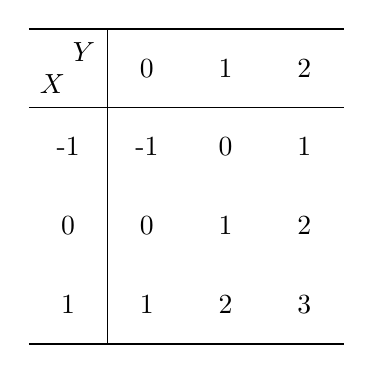
\begin{tikzpicture}
	\draw[thick](0,0)--(4,0) (0,-4)--+(4,0);
	\draw(0,-1)--+(4,0) (1,0)--+(0,-4);
	\draw(1.5,-.5)node{0}
		(2.5,-.5)node{1}
		(3.5,-.5)node{2}
		(.5,-1.5)node{-1}
		(.5,-2.5)node{0}
		(.5,-3.5)node{1}
		(.3,-.7)node{\(X\)}
		(.7,-.3)node{\(Y\)}
		(1.5,-1.5)node{-1}
		(2.5,-1.5)node{0}
		(3.5,-1.5)node{1}
		(1.5,-2.5)node{0}
		(2.5,-2.5)node{1}
		(3.5,-2.5)node{2}
		(1.5,-3.5)node{1}
		(2.5,-3.5)node{2}
		(3.5,-3.5)node{3};
\end{tikzpicture}
\end{center}
由此可知\(Z \in \Set{-1,0,1,2,3}\),那么
\def\sp#1{\sum_{x_i+y_j=#1} p_{ij}}
\begin{align*}
	&P(Z=-1) = \sp{-1} = \frac{1}{12}, \\
	&P(Z=0) = \sp{0} = \frac{1}{4}, \\
	&P(Z=1) = \sp{1} = \frac{5}{12}, \\
	&P(Z=2) = \sp{2} = \frac{1}{12}, \\
	&P(Z=3) = \sp{3} = \frac{1}{6},
\end{align*}
即\[
	Z \sim \begin{bmatrix}
		-1 & 0 & 1 & 2 & 3 \\
		\frac{1}{12} & \frac{1}{4} & \frac{5}{12} & \frac{1}{12} & \frac{1}{6}
	\end{bmatrix}.
\]
同理可得,\[
	W \sim \begin{bmatrix}
		0 & 1 & 2 \\
		\frac{1}{6} & \frac{1}{2} & \frac{1}{3}
	\end{bmatrix}.
\]
\end{solution}
\end{example}

\begin{theorem}\label{theorem:多维随机变量及其分布.离散型随机变量的卷积公式}
设二维离散型随机变量\((X,Y)\)有概率分布\(P(X=h,Y=k)\),
\(Z=X+Y\),则有\begin{align}
	P(Z=k)
	&= \sum_{r=0}^k P(X=r,Y=k-r) \\
	&= \sum_{r=0}^k P(X=k-r,Y=r).
\end{align}
特别地,当\(X\)与\(Y\)独立时,有\begin{align}
	P(Z=k)
	&= \sum_{r=0}^k P(X=r) \cdot P(Y=k-r) \label{equation:多维随机变量及其分布.离散型随机变量的卷积公式1} \\
	&= \sum_{r=0}^k P(X=k-r) \cdot P(Y=r). \label{equation:多维随机变量及其分布.离散型随机变量的卷积公式2}
\end{align}
\rm\cref{equation:多维随机变量及其分布.离散型随机变量的卷积公式1,%
equation:多维随机变量及其分布.离散型随机变量的卷积公式2}
称为“(离散型随机变量的)\DefineConcept{卷积公式}”.
\end{theorem}

\subsection{二维连续型随机变量函数的分布}
设\((X,Y)\)是二维连续型随机变量,且有密度函数\(f(x,y)\).
若\(g(x,y)\)是连续函数,
则\(Z = g(X,Y)\)是一维连续型随机变量.
\begin{enumerate}
	\item 首先根据\(X\)和\(Y\)的取值区间,确定\(Z\)的取值区间\(R(Z)\);

	\item 对任意\(z \in R(Z)\),
	求\(Z\)的分布函数\(F_Z(z)\),
	即\begin{align*}
		F_Z(z) &= P(Z \leq z)
		= P[g(X,Y) \leq z]
		= P[(X,Y) \in G(z)] \\
		&= \iint_{G(z)} f(x,y) \dd{x}\dd{y}.
	\end{align*}
	这里\(G(z) = \Set{ z\in\mathbb{R} \given g(x,y) \leq z }\).
	当\(z \notin R(Z)\)时,有\(F_Z(z)=0\)或\(F_Z(z)=1\).

	\item 求导得到\(Z\)的密度函数\(f_Z(z) = F'_Z(z)\).
\end{enumerate}

\begin{example}
设\((X,Y)\)的密度函数为\[
f(x,y) = \left\{ \begin{array}{cl}
xy, & 0 \leq x \leq 2, 0 \leq y \leq 1, \\
0, & \text{其他}.
\end{array} \right.
\]求\(Z = XY\)的密度.
\begin{solution}
\begin{figure}[ht]
	\centering
	\begin{tikzpicture}
		\begin{scope}[>=Stealth,->]
			\draw(0,0)node[below left]{\(O\)}--(3,0)node[below]{\(x\)};
			\draw(0,0)--(0,2)node[left]{\(y\)};
		\end{scope}
		\draw(0,1)node[left]{\(1\)}--(2,1)--(2,0)node[below]{\(2\)};
		\pgfmathsetmacro{\z}{1.5}
		\pgfmathsetmacro{\y}{\z/2}
		\draw[dashed](\z,0)node[below]{\(z\)}--(\z,1)node[above right]{\(xy=z\)};
		\pgfmathsetmacro{\a}{3*(2+\z)/4}
		\pgfmathsetmacro{\r}{.5*sqrt(2.5)*sqrt(4+\z^2)}
		\pgfmathsetmacro{\sx}{.8}
		\pgfmathsetmacro{\sy}{\a-sqrt(\r^2-(\sx-\a)^2)}
		\pgfmathsetmacro{\dx}{2.5}
		\pgfmathsetmacro{\dy}{\a-sqrt(\r^2-(\dx-\a)^2)}
		\draw(\sx,\sy)..controls(\z,.85)..(\dx,\dy);
	\end{tikzpicture}
	\caption{}
	\label{figure:多维随机变量及其分布.二维连续型随机变量函数的分布.例1}
\end{figure}
由题意有,\(Z\)的值域为\(R(Z)=[0,2]\).
如\cref{figure:多维随机变量及其分布.二维连续型随机变量函数的分布.例1},
对\(\forall z\in[0,2]\),有\begin{align*}
	F_Z(z) &= P(Z \leq z)
	= P(XY \leq z)
	= \iint_{xy \leq z} f(x,y) \dd{x}\dd{y} \\
	&= \int_0^z \dd{x} \int_0^1 xy \dd{y}
		+ \int_z^2 \dd{x} \int_0^{z/x} xy \dd{y} \\
	&= \frac{z^2}{4} + \frac{z^2}{2} (\ln2 - \ln z),
\end{align*}
于是\[
	f_Z(z) = F_Z'(z)
	= \left\{ \begin{array}{cl}
		z \ln(2/z), & 0<z\leq2, \\
		0, & \text{其他}.
	\end{array} \right.
\]
\end{solution}
\end{example}

\begin{example}
设\(X \sim U(0,1)\),\(Y \sim e(1)\),且\(X\)与\(Y\)相互独立,\(Z = X+Y\).
求\(Z\)的密度函数.
\begin{solution}
由题意有,\((X,Y)\)的密度函数为\[
	f(x,y) = \begin{cases}
		e^{-y}, & 0<x<1,y>0, \\
		0, & \text{其他};
	\end{cases}
\]
\(Z\)的值域为\(R(Z)=(0,+\infty)\).
对\(\forall z>0\),有\begin{align*}
	F_Z(z) &= P(Z \leq z) = P(X+Y \leq z) \\
	&= \iint_{x+y \leq z} f(x,y) \dd{x}\dd{y}.
\end{align*}
\begin{figure}
	\centering
	\begin{tikzpicture}
		\pgfmathsetmacro{\z}{2}
		\fill[black!30](0,0)--(\z,0)--(0,\z)--(0,0);
		\begin{scope}[>=Stealth,->]
			\draw(0,0)node[below left]{\(O\)}--(4,0)node[below]{\(x\)};
			\draw(0,0)--(0,4)node[left]{\(y\)};
		\end{scope}
		\draw(0,\z)--(\z,0)node[below]{\(z\)}
			node[pos=.1,above=5pt,right=5pt]{\(\begin{array}{l}
			x+y=z \\
			0<z<1
			\end{array}\)};
		\draw(3,0)node[below]{\(1\)}--(3,3);

		\begin{scope}[xshift=6cm]
		\pgfmathsetmacro{\z}{3.5}
		\fill[black!30](0,0)--(3,0)--(3,.5)--(0,0)
			(0,0)--(3,.5)--(0,3.5)--(0,0);
		\begin{scope}[>=Stealth,->]
			\draw(0,0)node[below left]{\(O\)}--(4,0)node[below]{\(x\)};
			\draw(0,0)--(0,4)node[left]{\(y\)};
		\end{scope}
		\draw(0,\z)--(\z,0)node[below]{\(z\)}
			node[pos=.1,above=5pt,right=5pt]{\(\begin{array}{l}
			x+y=z \\
			z\geq1
			\end{array}\)};
		\draw(3,0)node[below]{\(1\)}--(3,3);
		\end{scope}
	\end{tikzpicture}
	\caption{}
	\label{figure:多维随机变量及其分布.二维连续型随机变量函数的分布.例2}
\end{figure}
如\cref{figure:多维随机变量及其分布.二维连续型随机变量函数的分布.例2},
当\(0<z<1\)时,\begin{align*}
	F_Z(z) &= \int_0^z \dd{x} \int_0^{z-x} e^{-y} \dd{y} \\
	&= \int_0^z (1-e^{x-z}) \dd{x} \\
	&= z-1+e^{-z};
\end{align*}
当\(z\geq1\)时,\begin{align*}
	F_Z(z) &= \int_0^1 \dd{x} \int_0^{z-x} e^{-y} \dd{y} \\
	&= \int_0^1 (1-e^{x-z}) \dd{x} \\
	&= 1-e^{-z}(e-1).
\end{align*}
于是\[
	f_Z(z) = F'_Z(z)
	= \begin{cases}
		1 - e^{-z}, & 0<z<1, \\
		e^{-z}(e-1), & z\geq1, \\
		0, & \text{其他}.
	\end{cases}
\]
\end{solution}
\end{example}

\begin{example}
设\(X,Y\)独立同分布于\(U(0,1)\),\(Z=\frac{X}{Y}\),
求\(Z\)的密度函数.
\begin{solution}
由题意有,\((X,Y)\)的密度函数为\[
	f(x,y) = \begin{cases}
		1, & 0<x<1,0<y<1, \\
		0, & \text{其他};
	\end{cases}
\]
\(Z\)的值域为\(R(Z)=(0,+\infty)\).
对\(\forall z>0\),有\begin{align*}
	F_Z(z) &= P(Z \leq z) = P\left(\frac{X}{Y} \leq z\right) \\
	&= \iint_{\frac{x}{y} \leq z} f(x,y) \dd{x}\dd{y}.
\end{align*}
\begin{figure}
	\centering
	\begin{tikzpicture}
		\pgfmathsetmacro{\a}{3}
		\pgfmathsetmacro{\z}{.7}
		\fill[black!30](0,0)--(\z*\a,\a)--(0,\a)--(0,0);
		\begin{scope}[>=Stealth,->]
			\draw(0,0)node[below left]{\(O\)}--(4,0)node[below]{\(x\)}
				node[midway,below=.5cm]{\(\begin{array}[t]{l}
					x=yz \\
					0<z<1
					\end{array}\)};
			\draw(0,0)--(0,4)node[left]{\(y\)};
		\end{scope}
		\pgfmathsetmacro{\pb}{1.1*\a}
		\pgfmathsetmacro{\pa}{\pb*\z}
		\draw(0,0)--(\z*\a,\a)--(\pa,\pb);
		\draw[dashed](\z*\a,0)node[below]{\(z\)}--(\z*\a,\a);
		\draw(\a,0)node[below]{\(1\)}--(\a,\a)--(0,\a)node[left]{\(1\)};

		\begin{scope}[xshift=6cm]
			\pgfmathsetmacro{\z}{1.6}
			\fill[black!30](0,0)--(\a,\a/\z)--(0,\a)--(0,0)
				(0,\a)--(\a,\a)--(\a,\a/\z)--(0,\a);
			\begin{scope}[>=Stealth,->]
				\draw(0,0)node[below left]{\(O\)}--(4,0)node[below]{\(x\)}
					node[midway,below=.5cm]{\(\begin{array}[t]{l}
					x=yz \\
					z\geq1
					\end{array}\)};
				\draw(0,0)--(0,4)node[left]{\(y\)};
			\end{scope}
			\pgfmathsetmacro{\pa}{1.1*\a}
			\pgfmathsetmacro{\pb}{\pa/\z}
			\draw(0,0)--(\a,\a/\z)--(\pa,\pb);
			\draw[dashed](0,\a/\z)node[left]{\(\frac{1}{z}\)}--(\a,\a/\z);
			\draw(\a,0)node[below]{\(1\)}--(\a,\a)--(0,\a)node[left]{\(1\)};
		\end{scope}
	\end{tikzpicture}
	\caption{}
	\label{figure:多维随机变量及其分布.二维连续型随机变量函数的分布.例3}
\end{figure}
如\cref{figure:多维随机变量及其分布.二维连续型随机变量函数的分布.例3},
当\(0<z<1\)时,\[
	F_Z(z)
	= \int_0^z \dd{x} \int_{\frac{x}{z}}^1 \dd{y}
	= \frac{z}{2};
\]
当\(z\geq1\)时,\[
	F_Z(z)
	= \int_0^1 \dd{x} \int_{\frac{x}{z}}^1 \dd{y}
	= 1 - \frac{1}{2z}.
\]
于是\[
	f_Z(z) = F'_Z(z) = \def\arraystretch{1.5} \begin{cases}
		\frac{1}{2}, & 0<z<1, \\
		\frac{1}{2z^2}, & z\geq1, \\
		0, & \text{其他}.
	\end{cases}
\]
\end{solution}
\end{example}

\begin{theorem}\label{theorem:多维随机变量及其分布.连续型随机变量的卷积公式}
设二维连续型随机变量\((X,Y)\)有密度函数\(f(x,y)\),
\(Z=X+Y\),则对任意\(z \in R(Z)\),有\begin{align}
f_Z(z) &= \int_{-\infty}^{+\infty} f(x,z-x) \dd{x} \\
&= \int_{-\infty}^{+\infty} f(z-y,y) \dd{y}.
\end{align}
特别地,当\(X\)与\(Y\)独立时,有\begin{align}
f_Z(z) &= \int_{-\infty}^{+\infty} f_X(x) f_Y(z-x) \dd{x} \label{equation:多维随机变量及其分布.连续型随机变量的卷积公式1} \\
&= \int_{-\infty}^{+\infty} f_X(z-y) f_Y(y) \dd{y}. \label{equation:多维随机变量及其分布.连续型随机变量的卷积公式2}
\end{align}
\rm\cref{equation:多维随机变量及其分布.连续型随机变量的卷积公式1,%
equation:多维随机变量及其分布.连续型随机变量的卷积公式2}
称为“(连续型随机变量的)\DefineConcept{卷积公式}”.
\end{theorem}

\begin{example}
\((X,Y)\)有密度函数\[
	f(x,y) = \begin{cases}
		2-x-y, & 0<x<1,0<y<1, \\
		0, & \text{其他}.
	\end{cases}
\]
\(Z=X+Y\),求\(f_Z(z)\).
\begin{solution}
由题意有,\(Z\)的值域为\(R(Z)=(0,2)\).
对\(\forall z\in(0,2)\),
由\cref{theorem:多维随机变量及其分布.连续型随机变量的卷积公式},有\[
	f_Z(z) = \int_{-\infty}^{+\infty} f(x,z-x) \dd{x}.
\]
其中被积函数为\[
	f(x,z-x)
	= 2-x-(z-x)
	= 2-z,
	\quad
	0<x<1,0<y=z-x<1.
\]
\begin{figure}[ht]
	\centering
	\begin{tikzpicture}
		\pgfmathsetmacro{\a}{3}
		\fill[black!30](0,0)--(\a,\a)--(\a,2*\a)--(0,\a)--(0,0);
		\begin{scope}[>=Stealth,->]
			\draw(0,0)node[below left]{\(O\)}
				--(2*\a,0)node[below]{\(x\)}
				node[midway,below=.5cm]{\(\begin{array}[t]{l}
					0<x<1 \\
					x<z<1+x
				\end{array}\)};
			\draw(0,0)--(0,2.5*\a)node[left]{\(z\)};
		\end{scope}
		\draw(0,0)--(1.5*\a,1.5*\a)node[pos=.8,below right]{\(x=z\)};
		\draw(0,\a)node[left]{1}--(1.5*\a,2.5*\a)node[pos=.8,below right]{\(1+x=z\)};
		\draw(\a,0)node[below]{1}--(\a,2*\a)--(0,2*\a)node[left]{2};
	\end{tikzpicture}
	\caption{}
	\label{figure:多维随机变量及其分布.二维连续型随机变量函数的分布.例4}
\end{figure}

如\cref{figure:多维随机变量及其分布.二维连续型随机变量函数的分布.例4},
画出被积函数的定义区域\(0<x<1,x<z<1+x\).

当\(0<z<1\)时,\[
	f_Z(z) = \int_0^z (2-z) \dd{x} = z(2-z);
\]
当\(1\leq z<2\)时,\[
	f_Z(z) = \int_{z-1}^1 (2-z) \dd{x} = (2-z)^2.
\]
因此,\[
	f_Z(z) = \begin{cases}
		z(2-z), & 0<z<1, \\
		(2-z)^2, & 1\leq z<2, \\
		0, & \text{其他}.
	\end{cases}
\]
\end{solution}
\end{example}

\section{多维随机变量}

\subsection{多维随机变量的概念与定义}
\begin{definition}
设\(\AutoTuple{X}{n}\)是\(n\)个定义在同一样本空间\(\Omega\)上的随机变量,
则称\((\AutoTuple{X}{n})\)为\(n\)维\DefineConcept{随机变量}.
\end{definition}

\begin{definition}
设\((\AutoTuple{X}{n})\)为\(n\)维\DefineConcept{随机变量},
称\(n\)元函数\[
F(\AutoTuple{x}{n})
= P(X_1 \leq x_1,X_2 \leq x_2,\dotsc,X_n \leq x_n)
\]为\((\AutoTuple{X}{n})\)的\(n\)维\DefineConcept{分布函数}.
\end{definition}

\begin{definition}
记\(F_i(x_i)\)为\(X_i\)的边缘分布函数.
若对任意实数\(\AutoTuple{x}{n}\),有\[
F(\AutoTuple{x}{n}) = F_1(x_1) F_2(x_2) \dotsm F_n(x_n),
\]则称“随机变量\((\AutoTuple{X}{n})\) \DefineConcept{相互独立}”.
\end{definition}

\subsection{n维离散型随机变量}
\begin{definition}
若\((\AutoTuple{X}{n})\)是\(n\)个定义在同一样本空间\(\Omega\)上的离散型随机变量,
则称\((\AutoTuple{X}{n})\)为 \DefineConcept{\(n\)维离散型随机变量},且称\[
p_{i_1 i_2 \dotso i_n}
= P(X_1=x_{i_1},X_2=x_{i_2},\dotsc,X_n=x_{i_n}),
\quad i_1,i_2,\dotsc,i_n=1,2,\dotsc
\]为\((\AutoTuple{X}{n})\)的 \DefineConcept{\(n\)维概率分布}.
\end{definition}

\begin{property}
\(n\)维概率分布具有以下性质:
\begin{enumerate}
\item \(p_{i_1 i_2 \dotso i_n} \geq 0\);
\item \(\sum_{i_1,i_2,\dotsc,i_n}{p_{i_1 i_2 \dotso i_n}} = 1\).
\end{enumerate}
\end{property}

\begin{definition}
在\(N\)重独立试验中,若每次试验有\(n+1\)种可能结果\(A_1,A_2,\dotsc,A_{n+1}\),
且\[
	0<p_i=P(A_i)<1\ (i=1,2,\dotsc,n+1),
	\qquad
	\sum_{i=1}^{n+1}{p_i}=1.
\]
令\(X_i\)表示\(N\)重独立试验中\(A_i\ (i=1,2,\dotsc,n)\)发生的次数,
则\((\AutoTuple{X}{n})\)所服从的分布称为\DefineConcept{多项分布},
记为\((\AutoTuple{X}{n}) \sim M(N;p_1,p_2,\dotsc,p_n)\).
其概率分布为\[
P(X_1=k_1,X_2=k_2,\dotsc,X_n=k_n)
= \frac{N!}{k_1! k_2!\dotsm k_{n+1}!} p_1^{k_1} p_2^{k_2} \dotsm p_n^{k_n} p_{n+1}^{k_{n+1}},
\]
其中\(0 \leq k_i \leq N\ (i=1,2,\dotsc,n+1)\),
且\(k_1 + k_2 + \dotsb + k_n + k_{n+1} = N\).
\end{definition}

\subsection{n维连续型随机变量}
\begin{definition}
若有\(n\)元非负函数\(f(\AutoTuple{x}{n})\)存在,使得\(n\)维随机变量\[
\vb{\Xi} = (\AutoTuple{X}{n})
\]的分布函数表示为\[
F(\AutoTuple{x}{n})
= \int_{-\infty}^{x_1} \int_{-\infty}^{x_2} \dotsi \int_{-\infty}^{x_n}
	f(u_1,u_2,\dotsc,u_n) \dd{u_1} \dd{u_2} \dotsm \dd{u_n},
\]则称\((\AutoTuple{X}{n})\)是 \DefineConcept{\(n\)维连续型随机变量},称\(f\)为\(\vb{\Xi}\)的 \DefineConcept{\(n\)维概率密度函数}.
\end{definition}

\begin{property}
\(n\)维概率密度函数具有以下性质:
\begin{enumerate}
\item \(\forall \AutoTuple{x}{n};\quad f(\AutoTuple{x}{n}) \geq 0\);
\item \(\int_{-\infty}^{+\infty} \int_{-\infty}^{+\infty} \dotsi \int_{-\infty}^{+\infty} f(u_1,u_2,\dotsc,u_n) \dd{u_1} \dd{u_2} \dotsm \dd{u_n}\).
\end{enumerate}
\end{property}

\begin{theorem}
设\((\AutoTuple{X}{n})\)有\(n\)维密度函数\(f(\AutoTuple{x}{n})\),
\(X_i\)有边缘密度\(f_i(x_i)\ (i=1,2,\dotsc,n)\),则:
\(\AutoTuple{X}{n}\)相互独立的充分必要条件是\[
f(\AutoTuple{x}{n})
= f_1(x_1) f_2(x_2) \dotsm f_n(x_n).
\]
\end{theorem}

\begin{definition}
设\(G\)是\(\mathbb{R}^n\)中一个可求度量的区域,
当\(n\)维随机变量\((\AutoTuple{X}{n})\)有密度函数\[
f(\AutoTuple{x}{n}) = \left\{ \begin{array}{ll}
\frac{1}{m(G)}, & (\AutoTuple{x}{n}) \in G, \\
0, & \text{其他}, \\
\end{array} \right.
\]其中\(m(G)\)为\(G\)的度量,
称\((\AutoTuple{X}{n})\)服从\(G\)上的\DefineConcept{均匀分布}.
\end{definition}

\section{分布的可加性}
\begin{definition}
当\(\AutoTuple{X}{n}\)相互独立且具有同一类型分布时,
若\(X_1+X_2+\dotsb+X_n\)也服从这一类型的分布,
就称这种类型的分布具有\DefineConcept{可加性}.
\end{definition}

\subsection{二项分布的可加性}
\begin{theorem}\label{theorem:多维随机变量及其分布.二项分布的可加性1}
%@see: 《概率论与数理统计》(陈鸿建、赵永红、翁洋) P91. 定理3.11
\(X \sim B(n,p)\),
\(Y \sim B(m,p)\),
且\(X\)与\(Y\)相互独立,
则\[
	X+Y \sim B(n+m,p).
\]
\begin{proof}
记\(Z = X+Y\).
\(Z\)的取值为\([0,n+m]\cap\mathbb{N}\).
事件\((Z=k)\)可以表示为\[
	(Z=k)
	= \bigcup_{r=0}^k (X=r,Y=k-r)
	\quad(k=0,1,\dotsc,n+m).
\]
注意上式右端为\(k+1\)个两两互斥事件之并,
再注意到\(X\)与\(Y\)独立,
则\begin{align*}
	P(Z=k)
	&= \sum_{r=0}^k P(X=r,Y=k-r) \\
	&= \sum_{r=0}^k P(X=r) P(Y=k-r) \\
	&= \sum_{r=0}^k C_n^r p^r (1-p)^{n-r} \cdot C_m^{k-r} p^{k-r} (1-p)^{m-k+r} \\
	&= p^k (1-p)^{n+m-k} \sum_{r=0}^k C_n^r C_m^{k-r} \\
	&= C_{n+m}^k p^k (1-p)^{n+m-k},
	\quad k=0,1,\dotsc,n+m.
\end{align*}
于是\(Z \sim B(n+m,p)\).
\end{proof}
\end{theorem}

\begin{corollary}\label{theorem:多维随机变量及其分布.二项分布的可加性2}
%@see: 《概率论与数理统计》(陈鸿建、赵永红、翁洋) P92. 推论1
设\(X_i \sim B(n_i,p)\ (i=1,2,\dotsc,n)\),
且\(\AutoTuple{X}{n}\)相互独立,
则\[
	X_1+X_2+\dotsb+X_n \sim B\left(\sum_{i=1}^n n_i,p\right).
\]
\end{corollary}

\begin{corollary}\label{theorem:多维随机变量及其分布.二项分布的可加性3}
%@see: 《概率论与数理统计》(陈鸿建、赵永红、翁洋) P92. 推论2
设\(X_i\ (i=1,2,\dotsc,n)\)独立同分布于\(0-1\)分布\(B(1,p)\),则\[
	X_1+X_2+\dotsb+X_n \sim B(n,p).
\]
\end{corollary}

\subsection{泊松分布的可加性}
\begin{theorem}\label{theorem:多维随机变量及其分布.泊松分布的可加性1}
%@see: 《概率论与数理统计》(陈鸿建、赵永红、翁洋) P92. 定理3.12
设\(X \sim P(\lambda_1)\),
\(Y \sim P(\lambda_2)\),
且\(X\)与\(Y\)相互独立,
则\[
	X+Y \sim P(\lambda_1 + \lambda_2).
\]
\end{theorem}

\begin{corollary}\label{theorem:多维随机变量及其分布.泊松分布的可加性2}
%@see: 《概率论与数理统计》(陈鸿建、赵永红、翁洋) P92. 推论
设\(X_i \sim P(\lambda_i)\ (i=1,2,\dotsc,n)\),
且\(\AutoTuple{X}{n}\)相互独立,
则\[
	X_1+X_2+\dotsb+X_n \sim P\left(\sum_{i=1}^n \lambda_i\right).
\]
\end{corollary}

\subsection{\texorpdfstring{\(\Gamma\)分布的可加性}{伽马分布的可加性}}
\begin{theorem}\label{theorem:多维随机变量及其分布.伽马分布的可加性1}
%@see: 《概率论与数理统计》(陈鸿建、赵永红、翁洋) P93. 定理3.14
设随机变量\(X_i \sim \Gamma(\alpha_i,\beta)\ (i=1,2,\dotsc,n)\),
且\(\AutoTuple{X}{n}\)相互独立,
则\[
	X_1+X_2+\dotsb+X_n
	\sim
	\Gamma\left(\sum_{i=1}^n \alpha_i,\beta\right).
\]
\end{theorem}

\section{最大值、最小值的分布}
\begin{theorem}
设随机变量\(\AutoTuple{X}{n}\)相互独立,
且\(X_i\)有分布函数\(F_i(x_i)\ (i=1,2,\dotsc,n)\),
则最大值\(M=\max\{\AutoTuple{X}{n}\}\)的分布函数为
\begin{equation}
	F_M(x) = F_1(x) F_2(x) \dotsm F_n(x);
\end{equation}
最小值\(N=\min\{\AutoTuple{X}{n}\}\)的分布函数为
\begin{equation}
	F_N(x) = 1 - [1-F_1(x)][1-F_2(x)]\dotsm[1-F_n(x)].
\end{equation}
\begin{proof}
显然有:
\begin{align*}
	F_M(x) &= P(\max\{\AutoTuple{X}{n}\} \leq x) \\
	&= P(X_1 \leq x,X_2 \leq x,\dotsc,X_n \leq x) \\
	&= P(X_1 \leq x) P(X_2 \leq x) \dotsm P(X_n \leq x) \\
	&= F_1(x) F_2(x) \dotsm F_n(x); \\
	F_N(x) &= P(\min\{\AutoTuple{X}{n}\} \leq x) \\
	&= 1 - P(\min\{\AutoTuple{X}{n}\} > x) \\
	&= 1 - P(X_1 > x,X_2 > x,\dotsc,X_n > x) \\
	&= 1 - P(X_1 > x) P(X_2 > x) \dotsm P(X_n > x) \\
	&= 1 - [1-F_1(x)][1-F_2(x)]\dotsm[1-F_n(x)].
	\qedhere
\end{align*}
\end{proof}
\end{theorem}

\begin{corollary}
%@see: 《概率论与数理统计》(茆诗松、周纪芗、张日权) P137. 定理3.2.1
设随机变量\(\AutoTuple{X}{n}\)独立同分布,
它们的分布函数为\(F(x)\),密度函数为\(f(x)\).
那么这些随机变量的最大值\(M=\max\{\AutoTuple{X}{n}\}\)
和它们最小值\(N=\min\{\AutoTuple{X}{n}\}\)的分布函数分别为
\begin{gather}
	F_M(x) = [F(x)]^n, \\
	F_N(x) = 1-[1-F(x)]^n.
\end{gather}
\(M\)和\(N\)的密度函数分别为
\begin{gather}
	f_M(x) = n [F(x)]^{n-1} f(x), \\
	f_N(x) = n [1-F(x)]^{n-1} f(x).
\end{gather}
\end{corollary}

\begin{example}
设\(\AutoTuple{X}{n}\)独立同分布于\(U(0,1)\),求它们的最大值、最小值分布的分布函数.
\begin{solution}
均匀分布\(U(0,1)\)的分布函数为\[
F(x) = \left\{ \begin{array}{cc}
0, & x \leq 0, \\
x, & 0 < x < 1, \\
1, & x \geq 1.
\end{array} \right.
\]于是最大值\(M\)与最小值\(N\)的分布函数分别为\[
F_M(x) = \left\{ \begin{array}{cc}
0, & x \leq 0, \\
x^n, & 0 < x < 1, \\
1, & x \geq 1.
\end{array} \right.
\qquad
F_N(x) = \left\{ \begin{array}{cc}
0, & x \leq 0, \\
1-(1-x)^n, & 0 < x < 1, \\
1, & x \geq 1.
\end{array} \right.
\]
\end{solution}
\end{example}
